\documentclass[aspectratio=169]{beamer}
%\documentclass{beamer}
\usetheme{Madrid}


\usepackage{graphicx}
\usepackage[utf8]{inputenc}
\usepackage{hyperref}
\usepackage{listings}

%\setbeamertemplate{footline}[frame number]

\begin{document}

\title{Introduction to Neural Networks}  
\subtitle{Transfer learning} 
\author[J.I. Vasquez]{\textbf{Juan Irving Vásquez} \\jivg.org}
\date{\today \copyright}
\institute[jivg.org]{Centro de Innovación y Desarrollo Tecnológico en Cómputo \\ Instituto Politécnico Nacional}
\titlegraphic{
\includegraphics[width=2cm]{ipn-cidetec}}

\frame{\titlepage} 


%\frame{
%	\frametitle{Contents}
%	\tableofcontents
%}

%%%%%%%%%%%%%%%%%%%%%%%%%%%%%%%%%%%%%%%%%%%%%%%%%%%%%%%%


\begin{frame}[fragile]
\frametitle{Neural networks advances}
\begin{center}
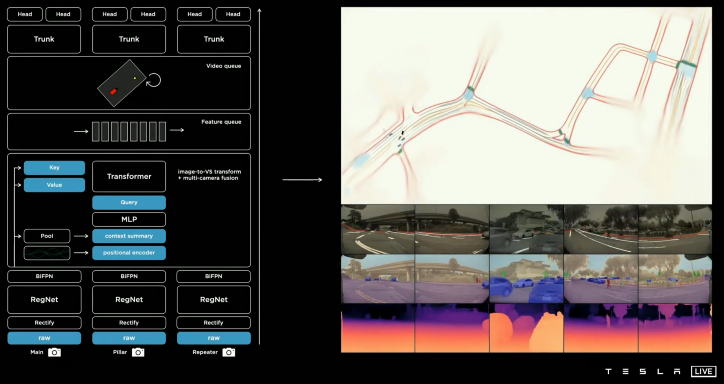
\includegraphics[width=0.9\linewidth]{./tesla}
\end{center}

\end{frame}


%\begin{frame}[fragile]
%\frametitle{Keras: The Python Deep Learning library}
%\begin{itemize}
%\item Keras is a high-level neural networks API, written in Python and capable of running on top of TensorFlow, CNTK, or Theano. 
%\item Fast experimentation.
%\item Being able to go from idea to result with the least possible delay is key to doing good research.
%\item Use Keras if you need a deep learning library that:
%\begin{itemize}
%\item Allows for easy and fast prototyping (through user friendliness, modularity, and extensibility).
%\item Supports both convolutional networks and recurrent networks, as well as combinations of the two.
%\item Runs seamlessly on CPU and GPU.
%\end{itemize}
%\end{itemize}
%\end{frame}



%\begin{frame}[fragile]
%\frametitle{Neural Networks in Keras}
%\begin{itemize}
%\item Here are some core concepts you need to know for working with Keras.
%
%\item Sequential Model
%\begin{verbatim}
%from keras.models import Sequential
%\end{verbatim}
%
%\item Create the Sequential model
%\begin{verbatim}
%model = Sequential()
%\end{verbatim}
%
%\item The keras.models.Sequential class is a wrapper for the neural network model. It provides common functions like fit(), evaluate(), and compile(). We'll cover these functions as we get to them. Let's start looking at the layers of the model.
%\end{itemize}
%\end{frame}


%\begin{frame}[fragile]
%\frametitle{Layers}
%{\scriptsize \begin{verbatim}
%from keras.models import Sequential
%from keras.layers.core import Dense, Activation, Flatten
%
%#Create the Sequential model
%model = Sequential()
%
%#1st Layer - Add a flatten layer
%model.add(Flatten(input_shape=(32, 32, 3)))
%
%#2nd Layer - Add a fully connected layer
%model.add(Dense(100))
%
%#3rd Layer - Add a ReLU activation layer
%model.add(Activation('relu'))
%
%#4th Layer - Add a fully connected layer
%model.add(Dense(60))
%
%#5th Layer - Add a ReLU activation layer
%model.add(Activation('relu'))
%\end{verbatim}}
%\end{frame}


%\begin{frame}[fragile]
%\frametitle{Review the following}
%\begin{itemize}
%\item Convolution
%\item Pooling
%\item Dropout
%\item Testing
%\end{itemize}
%\end{frame}


\frame{
	\frametitle{The reasons of success}
	\framesubtitle{Dataset sizes}
	\begin{figure}
		\centering
		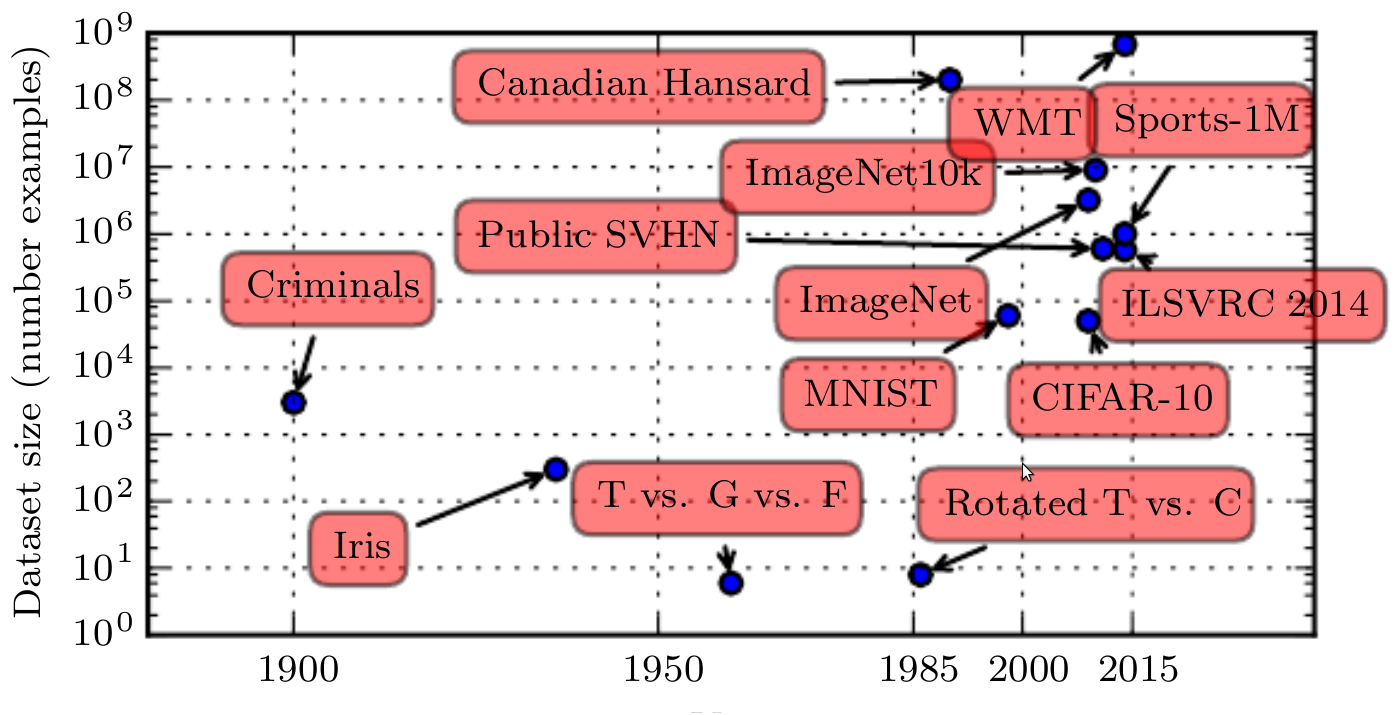
\includegraphics[height=0.7\textheight]{datasets}
		\caption{Dataset sizes over time}
		\label{fig:datasets}
	\end{figure}
}



\frame{
	\frametitle{The reasons of success}
	\framesubtitle{Dataset sizes}
	\begin{itemize}
		\item \url{https://image-net.org}
		\item \url{https://neurohive.io/en/datasets/tencent-dataset/}
		\item \url{http://xviewdataset.org/}
	\end{itemize}
}



\begin{frame}[fragile]
		\frametitle{The reasons of success}
		\framesubtitle{GPU proccessing times - Is it enough?}
\begin{center}
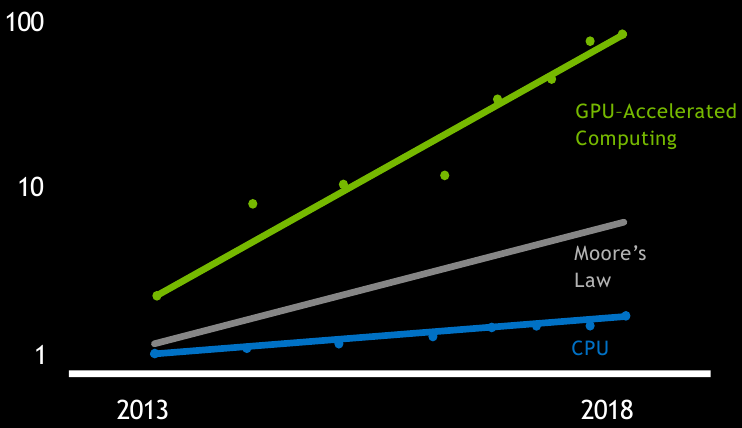
\includegraphics[height=0.7\textheight]{./nvidiaperformance_0}
\end{center}
\end{frame}


\frame{
	\frametitle{Practical problems}
	\begin{itemize}
		\item It is difficult to get data and computing power.
	\end{itemize}
\begin{center}
	
\includegraphics[height=0.7\textheight]{datasetmeme}
\end{center}		
}


{ 	\usebackgroundtemplate{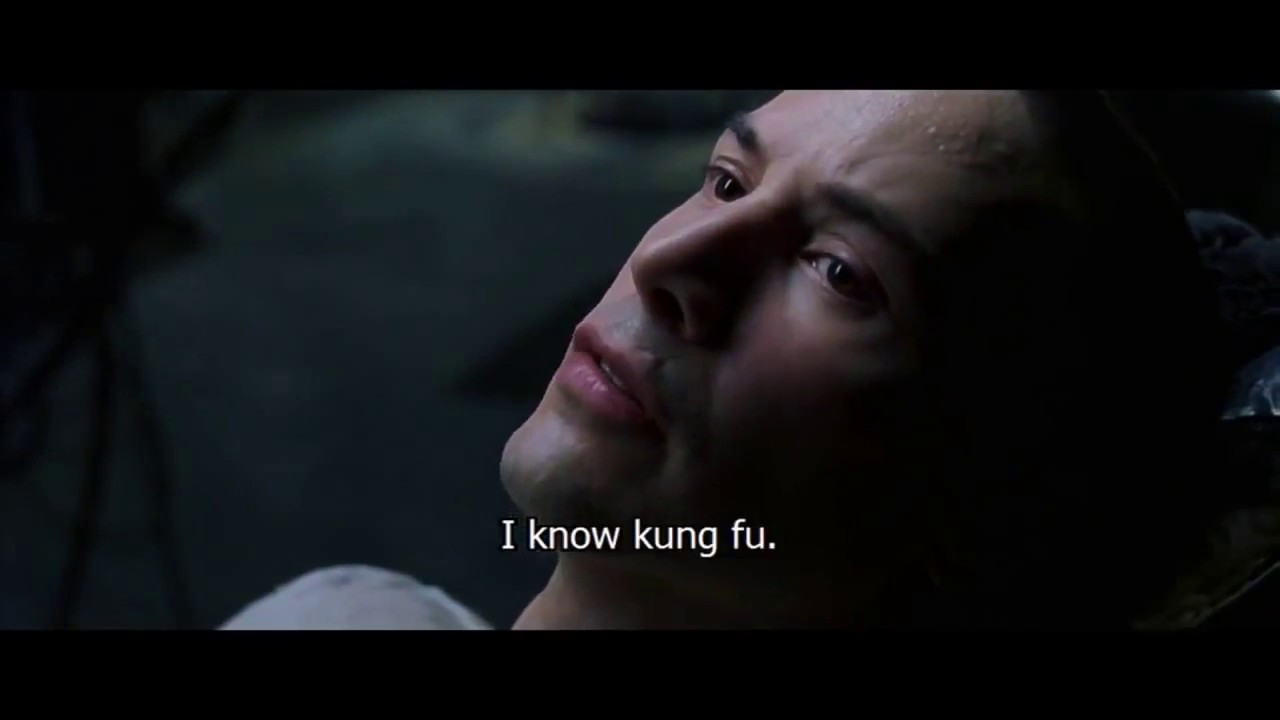
\includegraphics[width=1.17\paperwidth]{matrix}}%
\frame{
	\frametitle{Transfer Learning}
	\framesubtitle{"What has been learned in one sitting is exploited to improve generalization in another sitting"}
%	\begin{itemize}
%		\item "El que no oye consejo no llega a viejo"
%		\pause
%		\item "What has been learned in one sitting is exploited to improve generalization in another sitting"		
%	\end{itemize}
}
}


\frame{
	\frametitle{Transfer Learning}
	\begin{itemize}
		\item Many visual categories share low level notions.
\begin{center}
	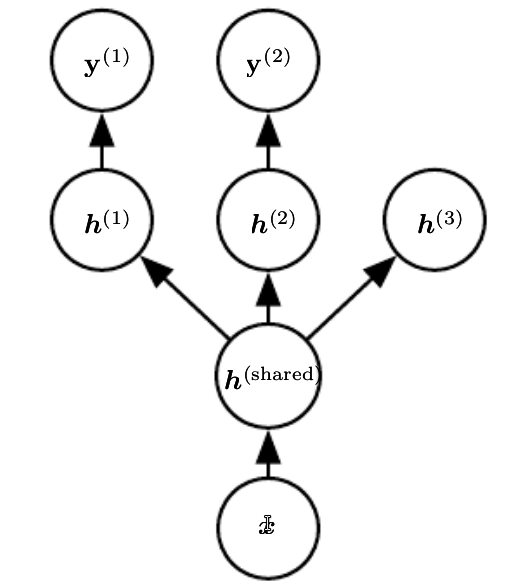
\includegraphics[height=0.6\textheight]{multitask}
\end{center}
	\end{itemize}
}


\frame{
	\frametitle{Transfer Learning}
	\begin{itemize}
		\item In some cases, the knowledge shared in on the top layers. e.g. speech recognition.
		\begin{center}
			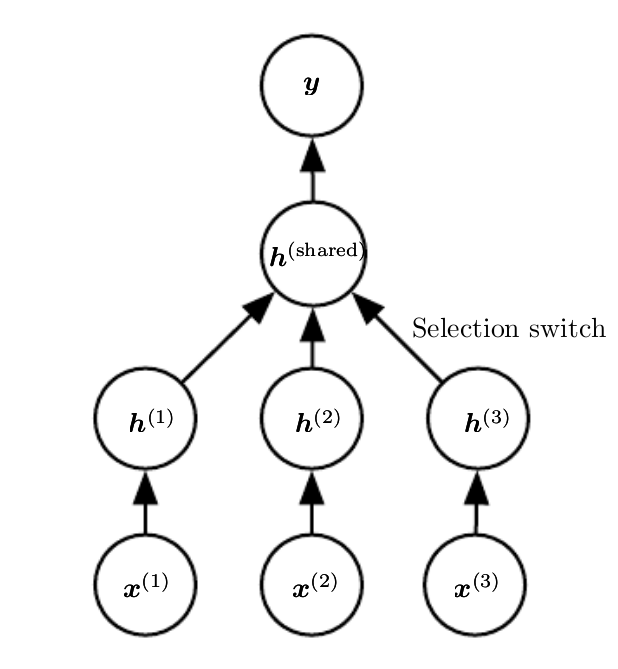
\includegraphics[height=0.6\textheight]{upshared}
		\end{center}
	\end{itemize}
}


\begin{frame}[fragile]
\frametitle{The Four Main Cases When Using Transfer Learning}
\begin{center}
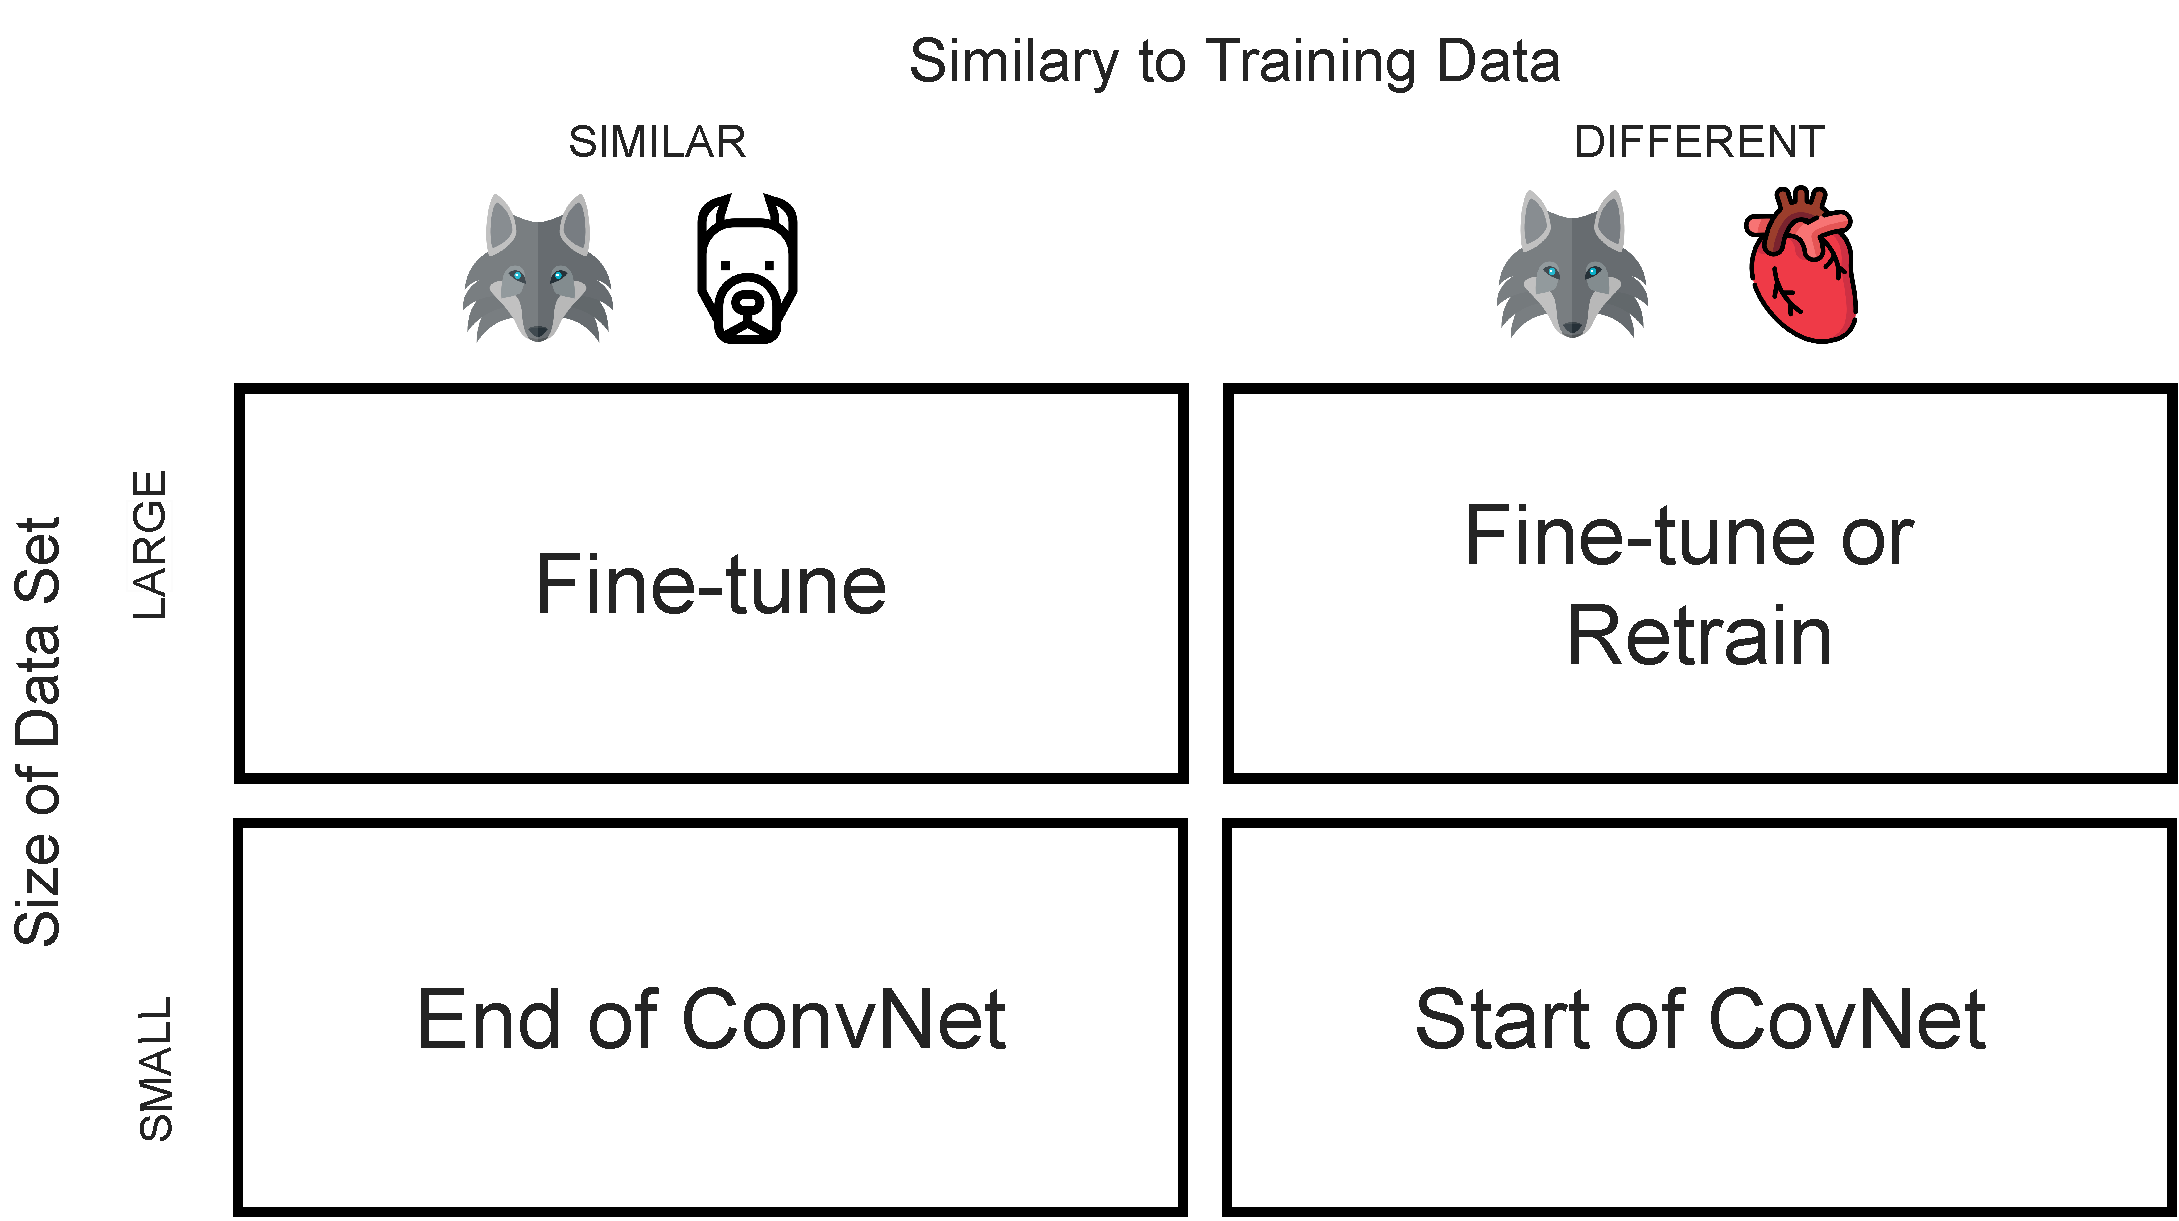
\includegraphics[height=0.7\textheight]{./transfer learning guide.drawio}
\end{center}
\end{frame}


\begin{frame}[fragile]
\frametitle{Demonstration network}
\framesubtitle{Pre-trained convolutional neural network}
\begin{center}
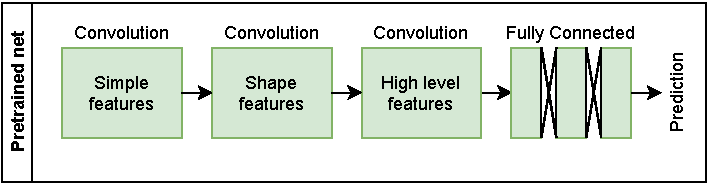
\includegraphics[width=0.7\linewidth]{./pretrained net-Page-1.drawio}
\end{center}
\end{frame}



\begin{frame}[fragile]
\frametitle{Case 1: Small Data Set, Similar Data}
\framesubtitle{Guide for How to Use Transfer Learning}
\begin{center}
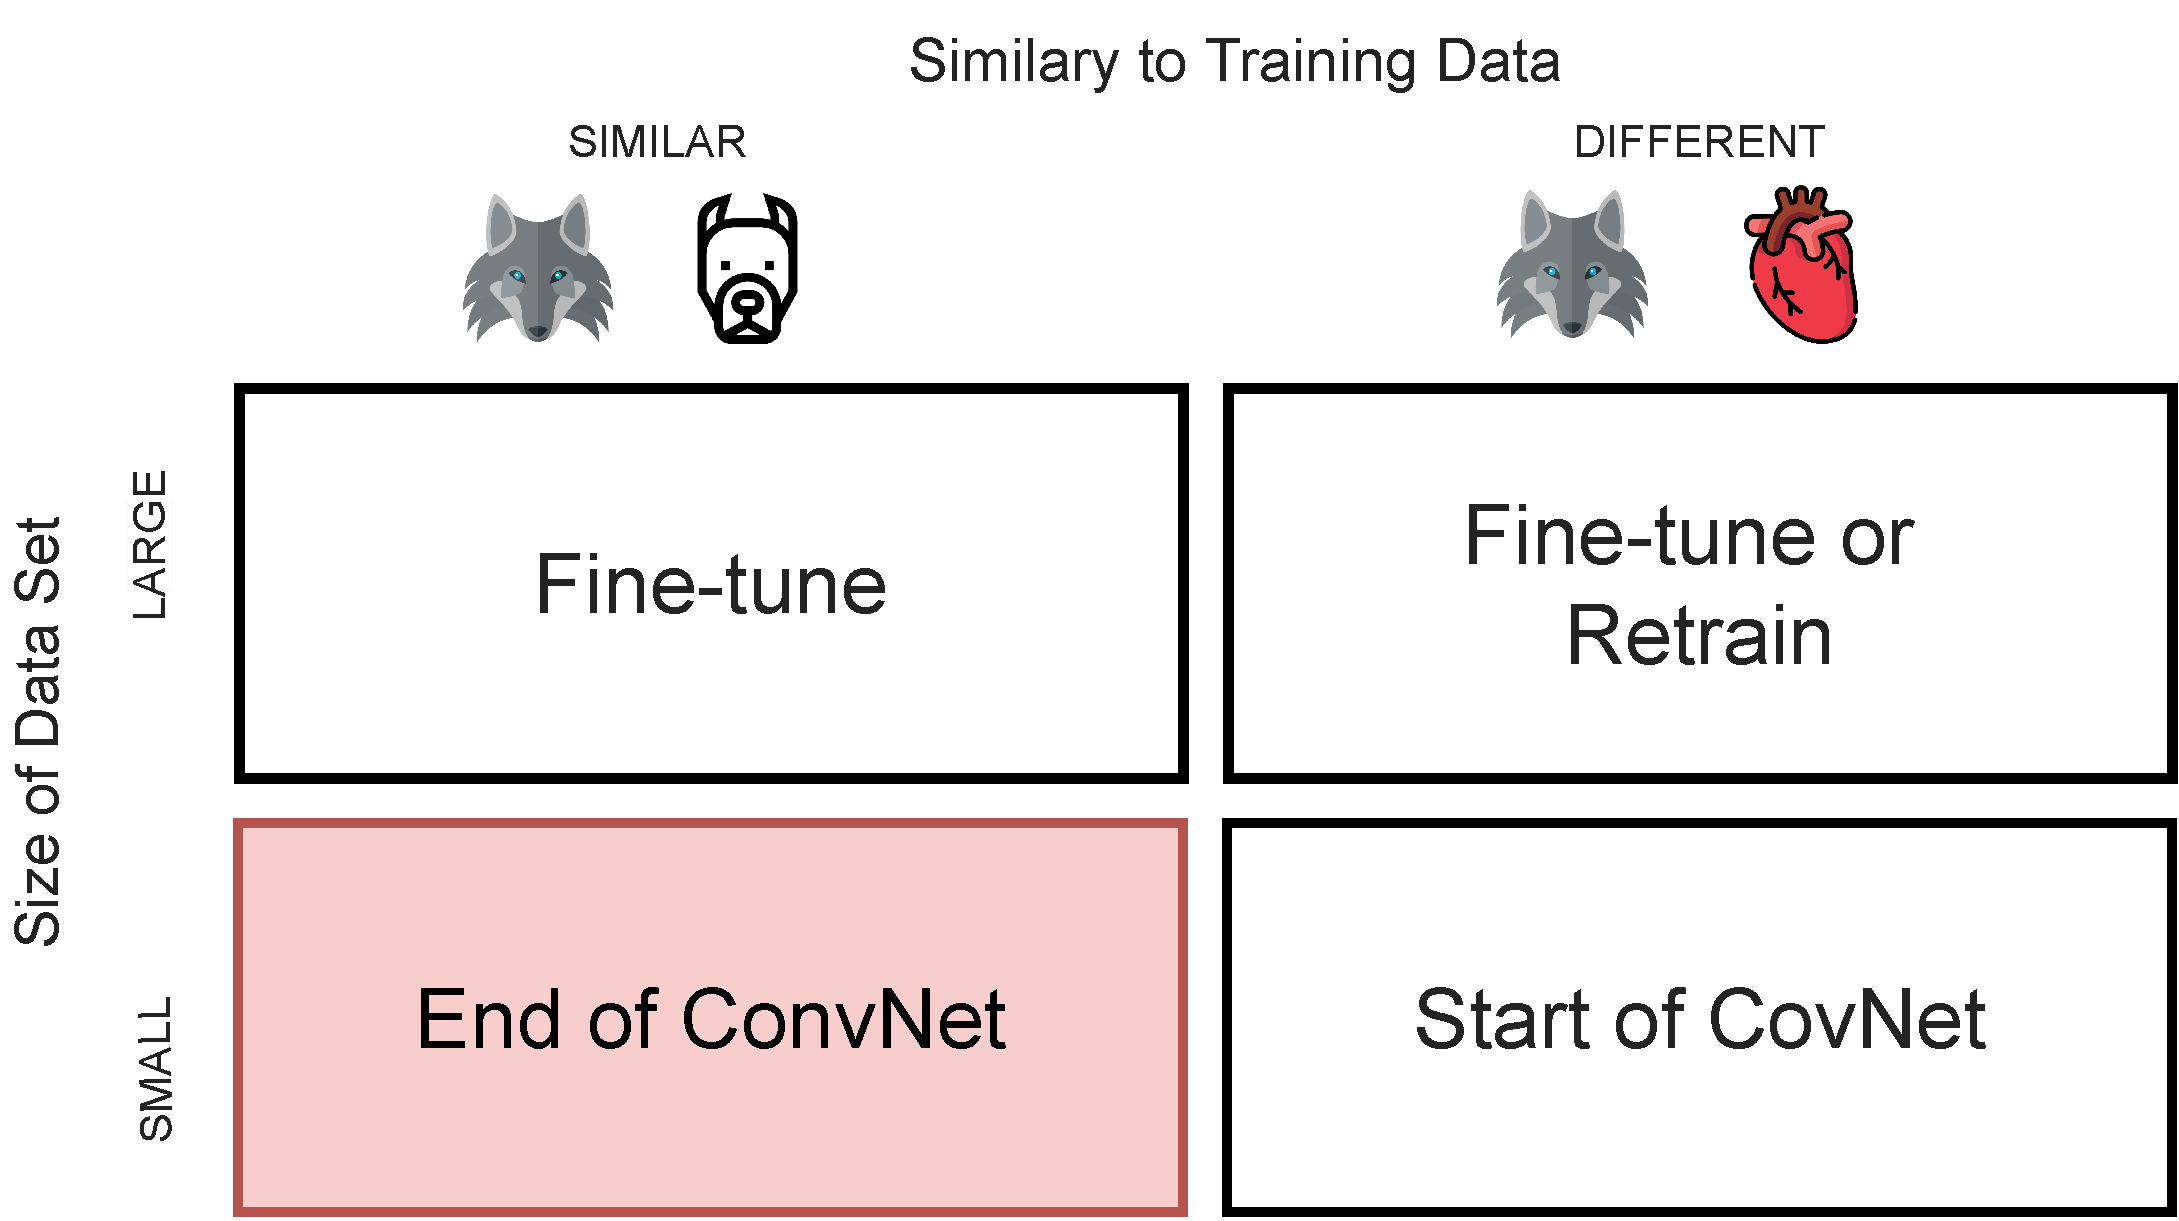
\includegraphics[height=0.7\textheight]{./transfer learning guide 21.drawio}
\end{center}
\end{frame}


\begin{frame}[fragile]
	\frametitle{Case 1: Small Data Set, Similar Data}
	\framesubtitle{Guide for How to Use Transfer Learning}
	\begin{center}
		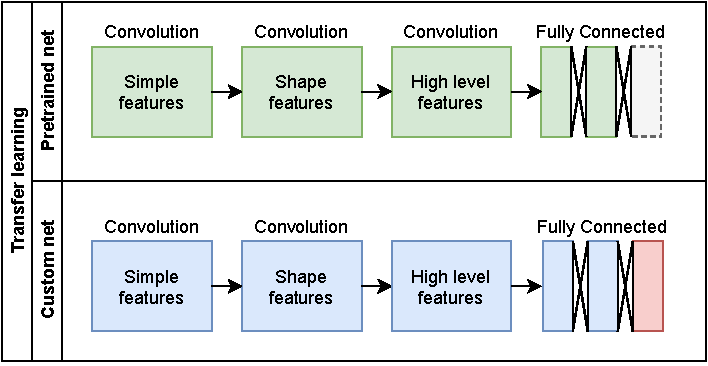
\includegraphics[width=0.7\linewidth]{./tl small ds similar-Page-1.drawio}
	\end{center}
\end{frame}



\begin{frame}[fragile]
\frametitle{Case 1: Small Data Set, Similar Data}
\framesubtitle{Guide for How to Use Transfer Learning}
If the new data set is small and similar to the original training data:
\begin{itemize}
\item slice off the end of the neural network
\item add a new fully connected layer that matches the number of classes in the new data set
\item randomize the weights of the new fully connected layer; freeze all the weights from the pre-trained network
\item train the network to update the weights of the new fully connected layer
\end{itemize}
To avoid overfitting on the small data set, the weights of the original network will be held constant rather than re-training the weights.
\end{frame}




\begin{frame}[fragile]
\frametitle{Case 2: Small Data Set, Different Data}
\framesubtitle{Guide for How to Use Transfer Learning}
\begin{center}
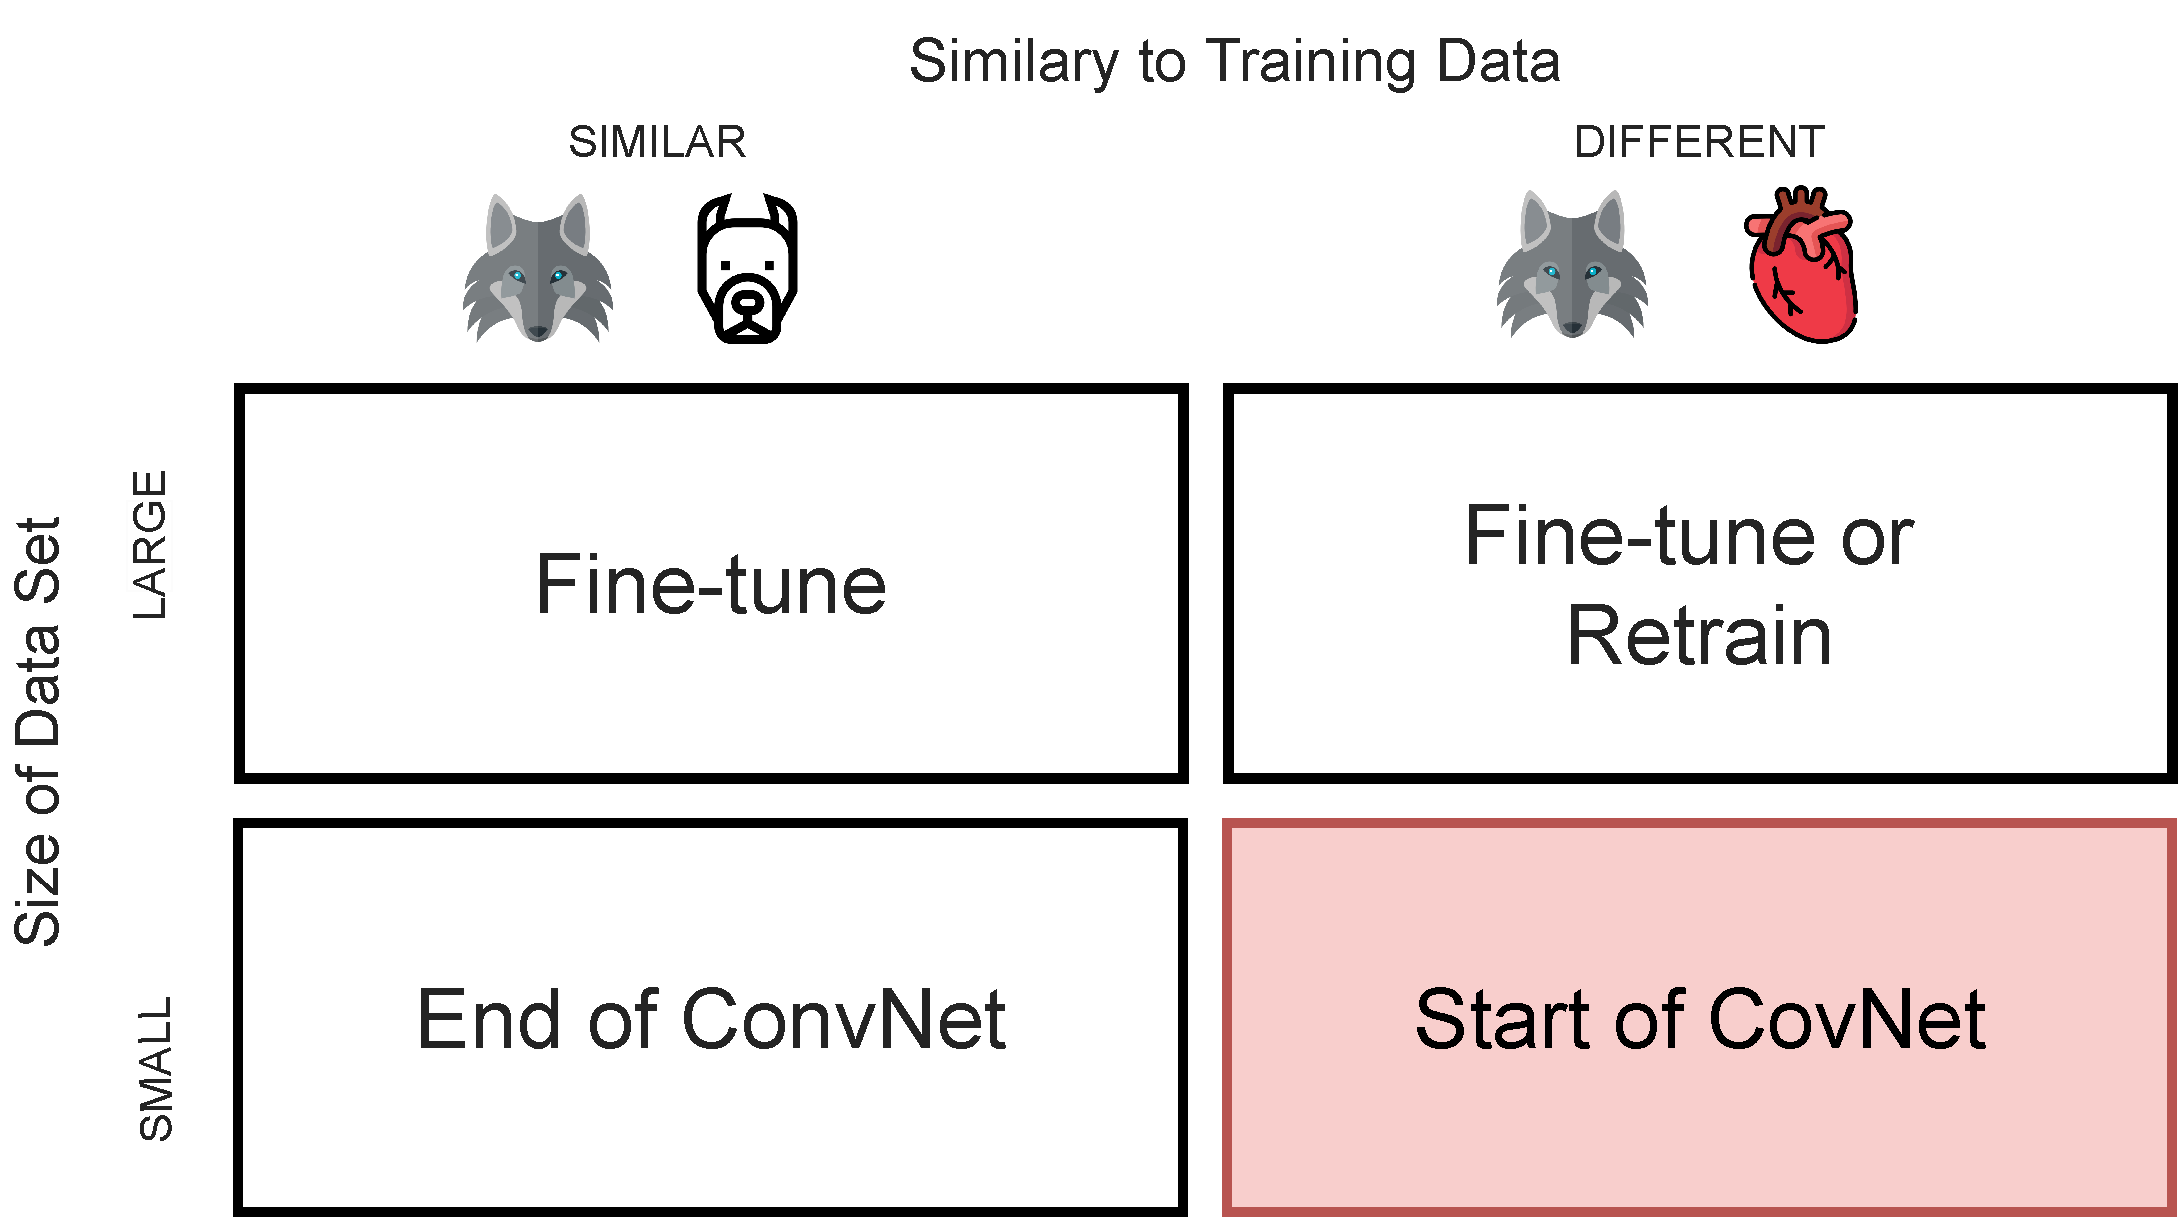
\includegraphics[height=0.7\textheight]{./transfer learning guide 22.drawio}
\end{center}
\end{frame}



\begin{frame}[fragile]
	\frametitle{Case 2: Small Data Set, Different Data}
	\framesubtitle{Guide for How to Use Transfer Learning}
	\begin{center}
		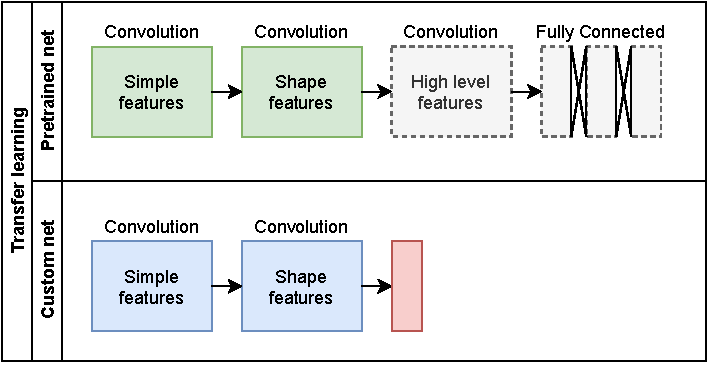
\includegraphics[width=0.7\linewidth]{./tl small ds different-Page-1.drawio}
	\end{center}
\end{frame}



\begin{frame}[fragile]
\frametitle{Case 2: Small Data Set, Different Data}
\framesubtitle{Guide for How to Use Transfer Learning}
If the new data set is small and different from the original training data:
\begin{itemize}
\item slice off most of the pre-trained layers near the beginning of the network
\item add to the remaining pre-trained layers a new fully connected layer that matches the number of classes in the new data set
\item randomize the weights of the new fully connected layer; freeze all the weights from the pre-trained network
\item train the network to update the weights of the new fully connected layer
\end{itemize}
Because the data set is small, overfitting is still a concern. To combat overfitting, the weights of the original neural network will be held constant, like in the first case.
\end{frame}



\begin{frame}[fragile]
\frametitle{Case 3: Large Data Set, Similar Data}
\framesubtitle{Guide for How to Use Transfer Learning}
\begin{center}
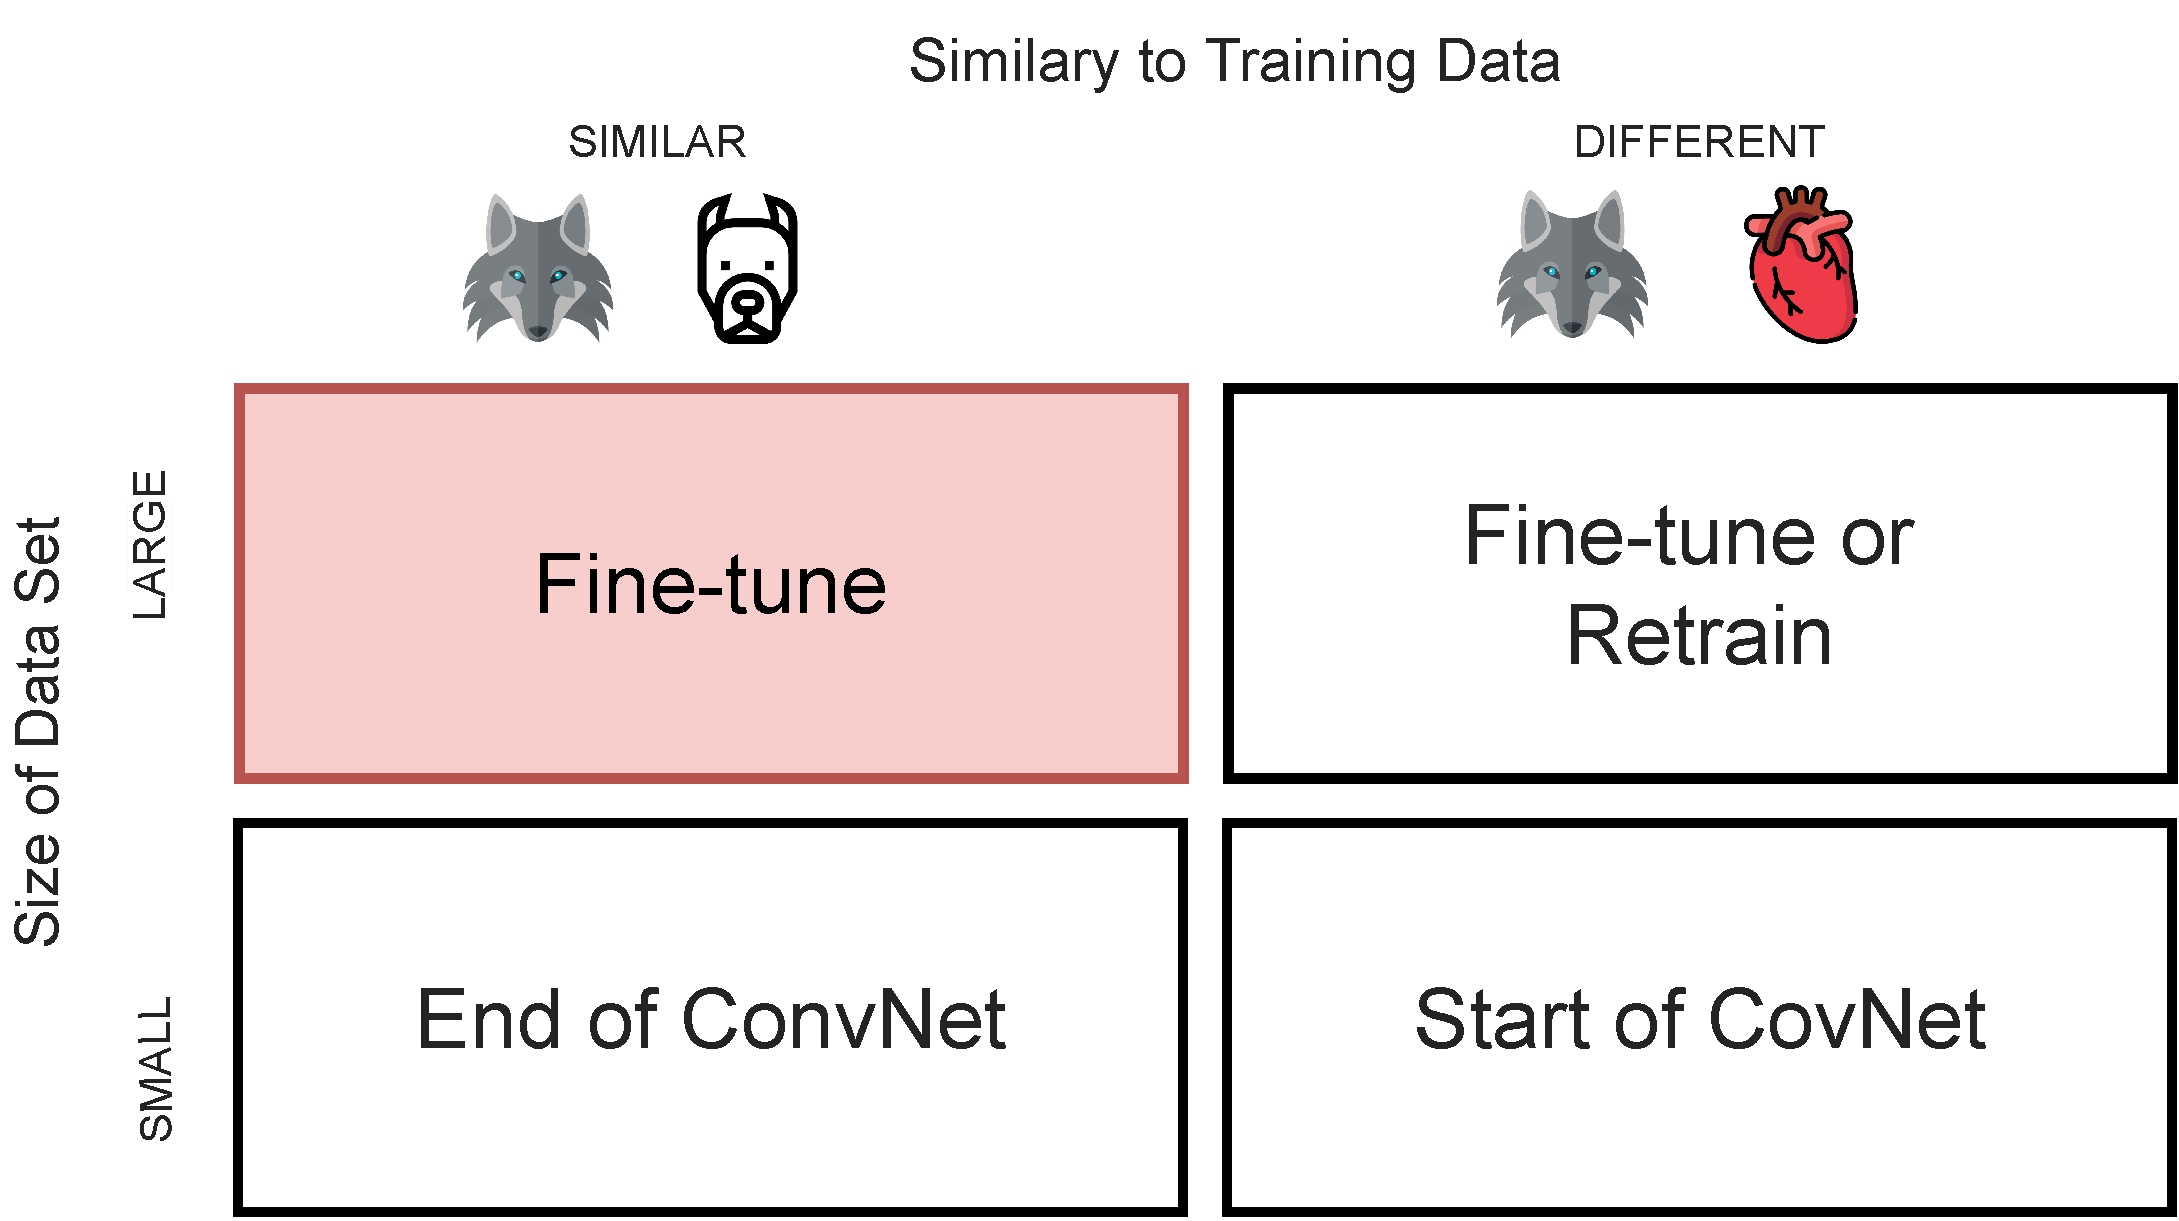
\includegraphics[height=0.7\textheight]{./transfer learning guide 11.drawio}
\end{center}
\end{frame}



\begin{frame}[fragile]
	\frametitle{Case 3: Large Data Set, Similar Data}
	\framesubtitle{Guide for How to Use Transfer Learning}
	\begin{center}
		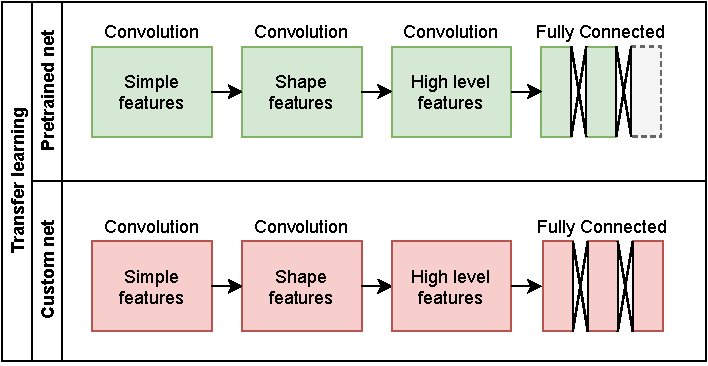
\includegraphics[width=0.7\linewidth]{./tl large ds similar-Page-1.drawio}
	\end{center}
\end{frame}



\begin{frame}[fragile]
\frametitle{Case 3: Large Data Set, Similar Data}
\framesubtitle{Guide for How to Use Transfer Learning}
If the new data set is large and similar to the original training data:
\begin{itemize}
\item remove the last fully connected layer and replace with a layer matching the number of classes in the new data set
\item randomly initialize the weights in the new fully connected layer
\item initialize the rest of the weights using the pre-trained weights
\item re-train the entire neural network
\end{itemize}
Overfitting is not as much of a concern when training on a large data set; therefore, you can re-train all of the weights.
\end{frame}




\begin{frame}[fragile]
\frametitle{Case 4: Large Data Set, Different Data}
\framesubtitle{Guide for How to Use Transfer Learning}
\begin{center}
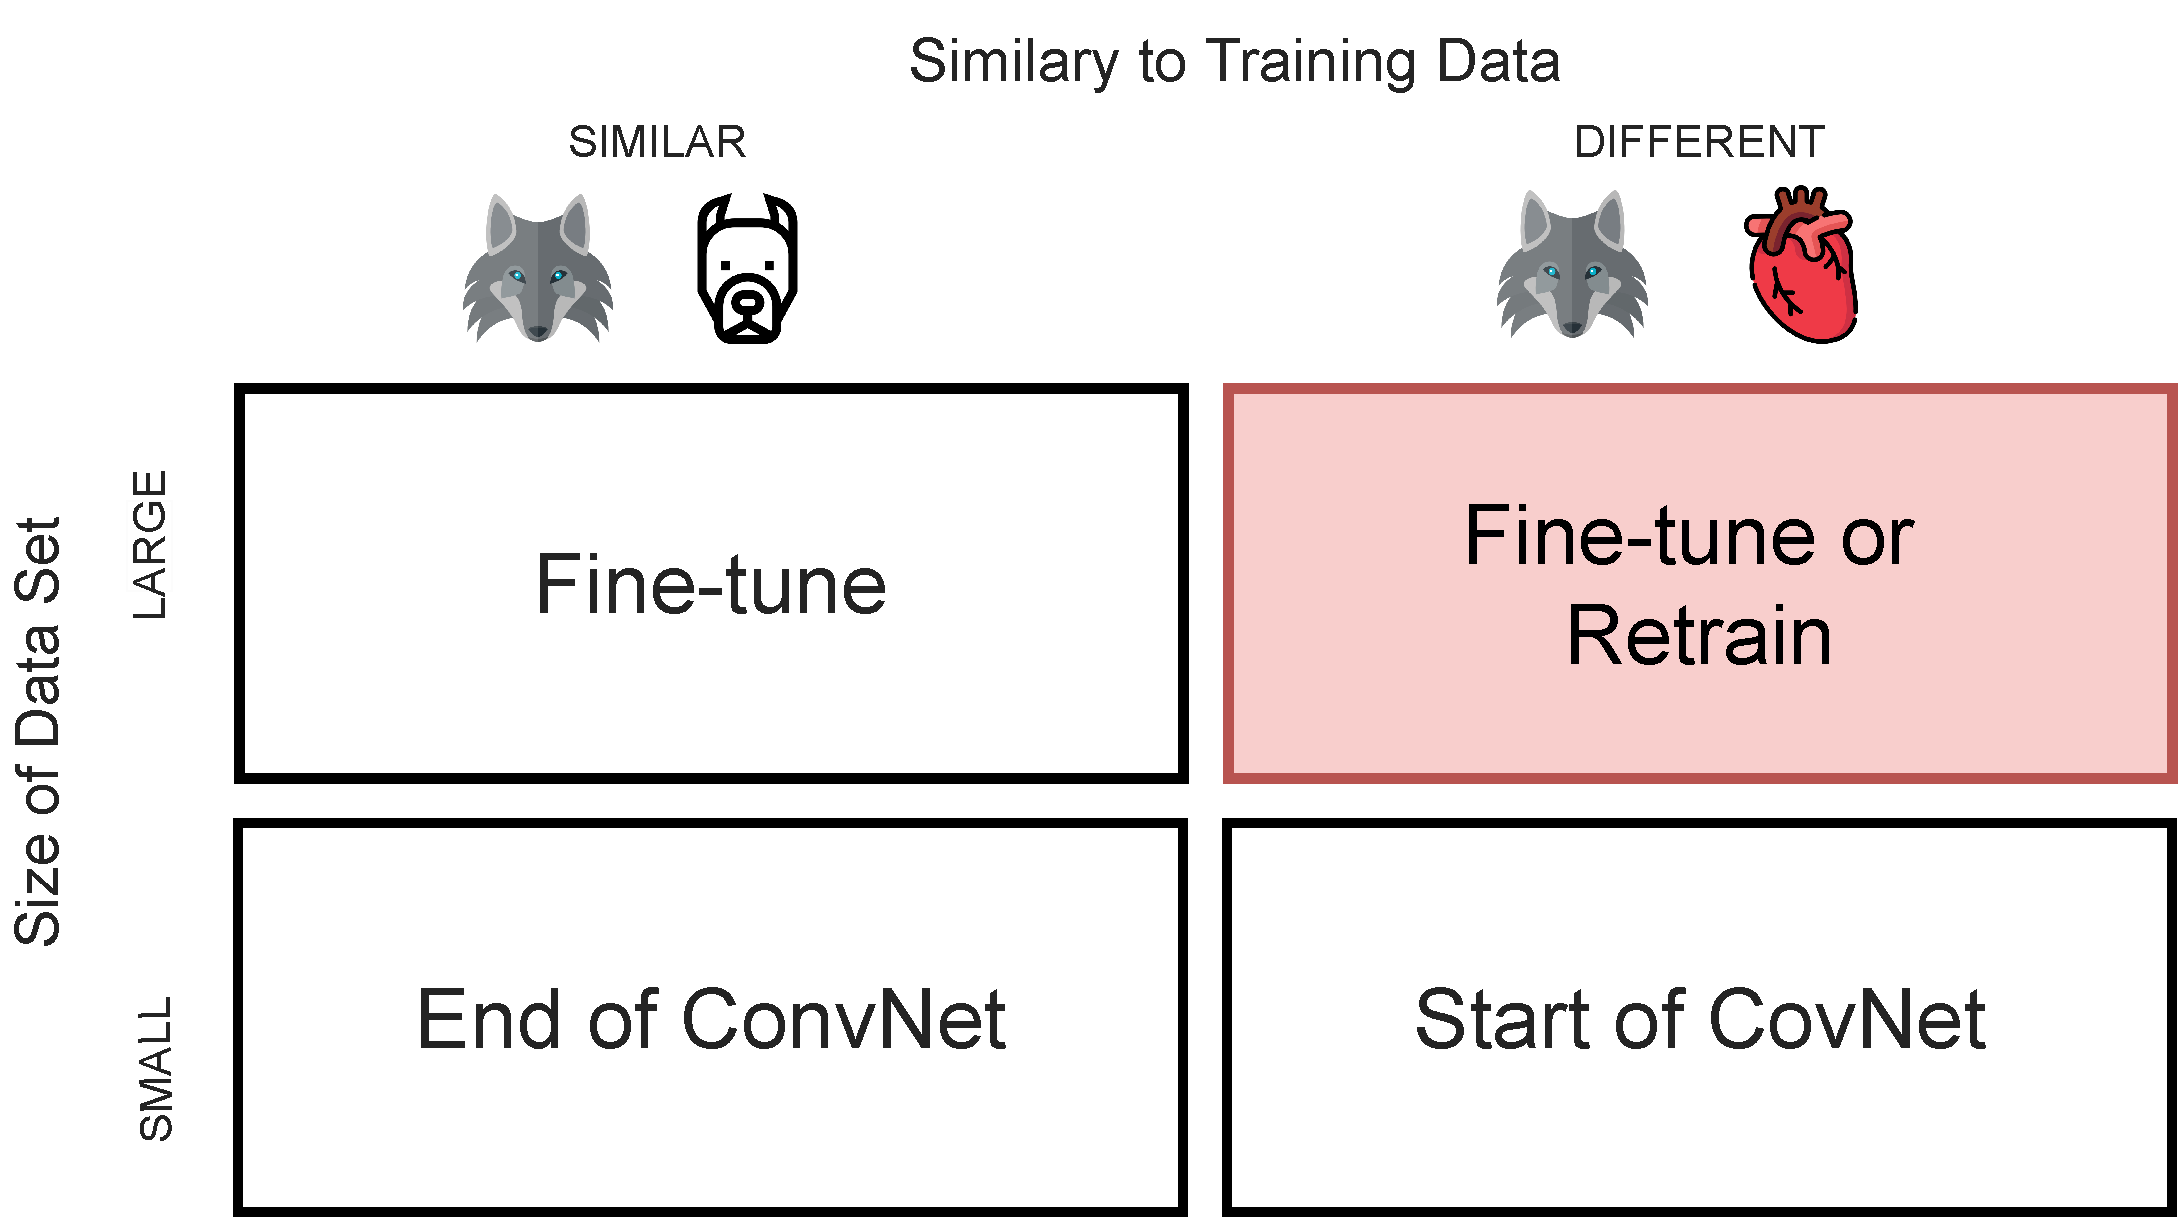
\includegraphics[height=0.7\textheight]{./transfer learning guide 12.drawio}
\end{center}
\end{frame}


\begin{frame}[fragile]
\frametitle{Case 4: Large Data Set, Different Data}
\framesubtitle{Guide for How to Use Transfer Learning}
If the new data set is large and different from the original training data:
\begin{itemize}
\item remove the last fully connected layer and replace with a layer matching the number of classes in the new data set
\item retrain the network from scratch with randomly initialized weights
\item alternatively, you could just use the same strategy as the "large and similar" data case
\end{itemize}
Even though the data set is different from the training data, initializing the weights from the pre-trained network might make training faster. So this case is exactly the same as the case with a large, similar data set.
\end{frame}



\begin{frame}[fragile]
\frametitle{Case 4: Large Data Set, Different Data}
\framesubtitle{Guide for How to Use Transfer Learning}
\begin{center}
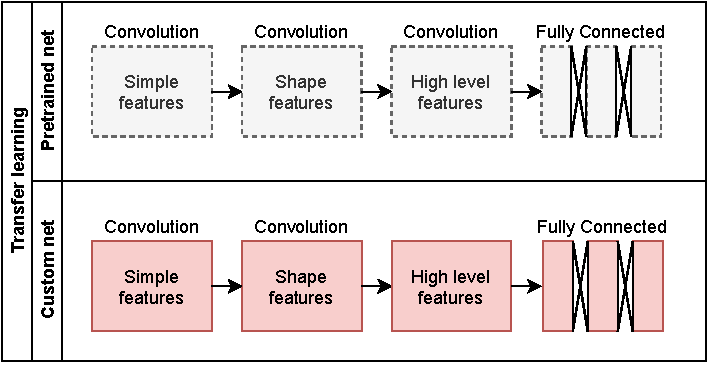
\includegraphics[width=0.7\linewidth]{./tl large ds different-Page-1.drawio}
\end{center}
\end{frame}



\begin{frame}[fragile]
\frametitle{Transfer learning}
\begin{center}
	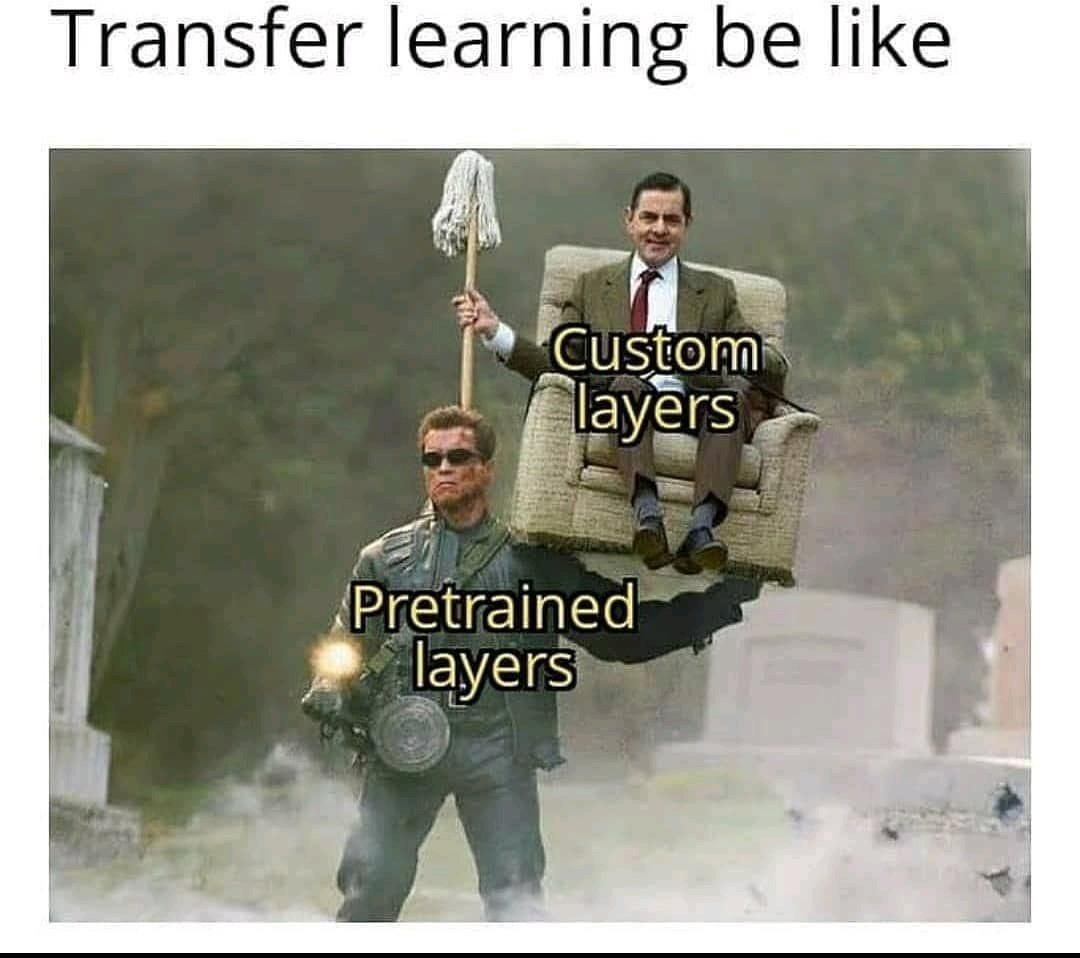
\includegraphics[height=0.8\textheight]{tlmeme}
\end{center}
\end{frame}



\begin{frame}[fragile]
\frametitle{One-shot learning}
\begin{itemize}
	\item Only one labeled example of the transfer task is given for one-shot learning.
	\item E.g. consider the problem of having a learner read a large collection of text and then solve object recognition problems.
	\item The model is trained to estimate the conditional distribution $p(y | x , T )$. where $T$ is a random variable describing the task. 
\end{itemize}
\end{frame}


\frame{
\frametitle{One-shot learning}
\begin{center}
	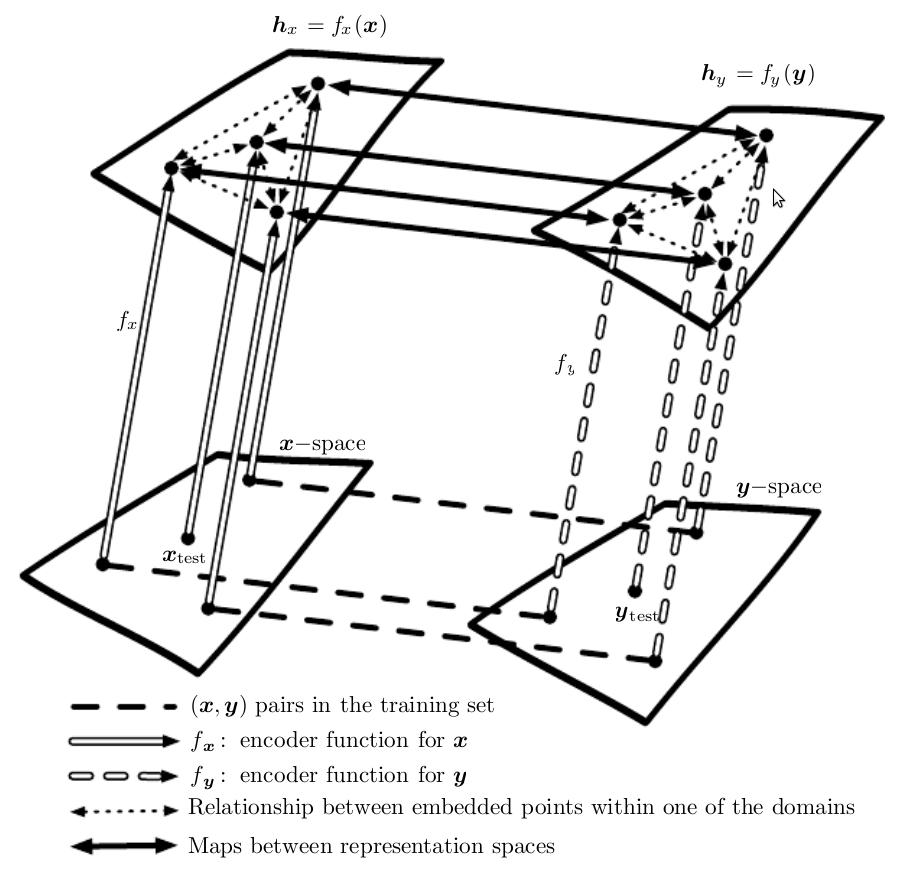
\includegraphics[width=0.5\linewidth]{zeroshot}
\end{center}
}


\frame{
\frametitle{References}
\begin{itemize}
\item [Goodfellow] Goodfellow, I., Bengio, Y., Courville, A., \& Bengio, Y. (2016). Deep learning (Vol. 1). Cambridge: MIT press.
\item [Sucar 15] Sucar, Luis Enrique. Probabilistic Graphical Models: Principles and Applications. Springer, 2015.
\item [Smola] Alex Smola and S.V.N. Vishwanathan, Introduction to Machine Learning, Cambirdge University Press.
\item [Udacity] Self Driving Car Nanodegree
\end{itemize}

}


\end{document}